\newpage

\section{Theory}
\label{sec:theory}

% ----------------------------
%  Motivation
% ----------------------------
\subsection{Motivation}
\label{subsec:motivation}

The shock angle \(\beta\) is a key parameter in the analysis of supersonic flows, as it determines the region of influence of disturbances and the behavior of shock waves. It is defined as the angle between the shock wave and the direction of the incoming flow, and it depends on the Mach number of the flow and the angle of attack of the object generating the shock.
\begin{equation}
    M_{n1} = M_\infty \sin\beta
\end{equation}
\vspace{4pt}
\begin{minipage}{0.48\linewidth}
\textit{(a) Pressure behind the shock}
\[
    \frac{p_2}{p_\infty}
    = 1 + \frac{2\gamma}{\gamma + 1}\bigl(M_{n1}^2 - 1\bigr),
\]
\end{minipage}
\hfill
\begin{minipage}{0.48\linewidth}
\textit{(b) Local pressure coefficient}
\[
    C_{p,2}
    = \frac{p_2 - p_\infty}{\tfrac{1}{2}\,\gamma\,p_\infty\,M_\infty^2}
    = \frac{2}{\gamma\,M_\infty^{2}}
    \Bigl(\tfrac{p_2}{p_\infty} - 1\Bigr).
\]
\end{minipage}

Knowing the Mach angle allows us to verify the validity of both the theoretical predictions and the numerical method.

In the \emph{small‐disturbance limit} (\(\theta \ll 1\), \(\beta \approx \mu\)), these expressions reduce to the familiar linear results:
\[
    C_p \approx \frac{2\theta}{\sqrt{M_\infty^{2} - 1}},
    \qquad
    C_L \approx -\,\frac{2\theta^{2}}{\sqrt{M_\infty^{2} - 1}},
    \qquad
    C_D \approx \frac{2\theta^{2}}{\sqrt{M_\infty^{2} - 1}}.
\]

% ----------------------------
%  Hypotheses
% ----------------------------
\subsection{Hypotheses}
\label{subsec:hypotheses}

\begin{itemize}
\item Inviscid, adiabatic, perfect-gas, steady flow:
    \begin{equation*}
        P = \rho R T, \quad \gamma = \mathrm{const}, \quad \nabla \cdot \boldsymbol{v} = 0, \quad \frac{\partial}{\partial t} = 0.
    \end{equation*}

\item Small perturbations of the flow field:
    \begin{equation*}
        \boldsymbol{v} = \boldsymbol{v}_0 + \boldsymbol{v}', \quad
        P = P_0 + P', \quad
        T = T_0 + T'.
    \end{equation*}

\item Expansion in disturbance amplitude:
    \begin{equation*}
        \boldsymbol{v}' = \epsilon\,\boldsymbol{v}_1 + \epsilon^2\,\boldsymbol{v}_2 + \epsilon^3\,\boldsymbol{v}_3 + \dots,
        \quad \epsilon \ll 1.
    \end{equation*}
\end{itemize}

% ----------------------------
%  Governing equations
% ----------------------------
\subsection{Governing equations}
\label{subsec:governing_equations}

The full compressible potential equation, a second‐order partial differential equation, can be written in terms of the velocity potential \(\phi\) as:
\begin{equation}
    (1 - M^2 \phi_x^2)\,\phi_{xx}
    - 2 M^2 \phi_x \phi_y \phi_{xy}
    + (1 - M^2 \phi_y^2)\,\phi_{yy}
    + \phi_{zz}
    = 0,
    \label{eq:governing_equations}
\end{equation}
where \(M\) is the Mach number, and \(\phi_x\), \(\phi_y\), and \(\phi_z\) denote the partial derivatives of \(\phi\) with respect to \(x\), \(y\), and \(z\), respectively.

\subsection{Linearized equations}
\label{subsec:linearized_equations}

By substituting the perturbation velocities into the governing equation \eqref{eq:governing_equations} and neglecting higher‐order terms, one obtains the linearized potential equation:
\begin{equation}
    (1 - M_\infty^2)\,\phi_{xx}
    + \phi_{yy}
    + \phi_{zz} = 0.
    \label{eq:small-disturb}
\end{equation}
This approximation omits all terms of order \(O(\phi_x^2)\) and above, as well as any shock–shock interactions, thereby limiting its validity to moderate Mach numbers and small deflection angles.

% ----------------------------
%  Shock angle
% ----------------------------
\subsection{Shock angle}

% ----- Exact relation -----
\subsubsection{Exact relation}

The exact oblique‐shock relation for a wedge half‐angle \(\theta\) is given in \emph{NASA Technical Paper 1406}:
\begin{equation}
    \tan\theta
    = 2 \cot\beta
      \,\frac{M_\infty^2 \sin^2\beta - 1}
            {M_\infty^2(\gamma + \cos 2\beta) + 2}.
    \label{eq:shock_angle}
\end{equation}
This equation cannot be solved analytically for \(\beta\) in terms of \(\theta\) and \(M_\infty\). In fact, it is a transcendental equation. However, one may apply the bisection method to find its solution numerically.

% ----- Numerical solution -----
\subsubsection{Numerical solution}

As mentioned above, equation \eqref{eq:shock_angle} has no closed‐form solution for \(\beta\). We therefore employ the bisection method, a simple and robust root‐finding algorithm for continuous functions, to compute \(\beta\) for a given \(\theta\) and \(M_\infty\).

Below is the Python code structured into functions, each handling a specific step of the solution process:

\begin{enumerate}[label=-, leftmargin=*, itemsep=1em]
    \item \textbf{Compute \(\theta\) from \(\beta\):}\\
    \texttt{theta\_from\_beta(beta, M, gamma)} evaluates
    \[
        \theta = \arctan\!\Biggl(
            \frac{2\,\cot\beta\,\bigl(M^2\sin^2\beta - 1\bigr)}
                 {M^2\bigl(\gamma + \cos2\beta\bigr) + 2}
        \Biggr).
    \]
    \begin{pycode}
def theta_from_beta(beta, M, gamma=1.4):
    """
    Returns theta (rad) for an oblique shock.
    Accepts beta as scalar or numpy array.
    """
    beta = np.asarray(beta)
    term1 = 2.0 / np.tan(beta)
    term2 = M**2 * np.sin(beta)**2 - 1.0
    term3 = M**2 * (gamma + np.cos(2.0*beta)) + 2.0
    return np.arctan(term1 * term2 / term3)
    \end{pycode}

    \item \textbf{Bisection method:}\\
    \texttt{bisection(beta\_low, beta\_high, f, tol, max\_iter)} solves
    \[
        f(\beta) = \theta(\beta) - \theta_{\mathrm{target}} = 0
    \]
    by iteratively halving the bracket \([\beta_{\mathrm{low}},\beta_{\mathrm{high}}]\).
    \begin{pycode}
def bisection(beta_low, beta_high, f, tol=1e-10, max_iter=100):
    """Find root of f(beta)=0 using bisection (beta in rad)."""
    f_low = f(beta_low)
    for _ in range(max_iter):
        beta_mid = 0.5*(beta_low + beta_high)
        f_mid = f(beta_mid)
        if abs(f_mid) < tol:
            return beta_mid
        if f_low * f_mid < 0.0:
            beta_high = beta_mid
        else:
            beta_low, f_low = beta_mid, f_mid
    raise RuntimeError("Bisection did not converge.")
    \end{pycode}

    \item \textbf{Bracket finding:}\\
    \texttt{bracket\_roots(theta\_rad, M, gamma, n\_scan)} scans \(\beta\) from
    \(\sin^{-1}(1/M)\) to \(89.9^\circ\) to locate sign changes in
    \(f(\beta)\), yielding intervals that contain roots.
    \begin{pycode}
def bracket_roots(theta_rad, M, gamma=GAMMA, n_scan=4000):
    beta_min = math.asin(1.0/M) + 1e-6
    beta_max = math.radians(89.9)
    betas = np.linspace(beta_min, beta_max, n_scan)
    f_vals = theta_from_beta(betas, M, gamma) - theta_rad
    idx = np.where(np.diff(np.sign(f_vals)))[0]
    return [(betas[i], betas[i+1]) for i in idx]
    \end{pycode}

    \item \textbf{Compute \(\beta\) solutions:}\\
    \texttt{beta\_solutions(theta\_deg, M, gamma)} converts \(\theta\) to radians,
    identifies brackets, and applies the bisection method to return
    weak and (optionally) strong‐shock angles.
    \begin{pycode}
def beta_solutions(theta_deg, M, gamma=GAMMA):
    theta_rad = math.radians(theta_deg)
    intervals = bracket_roots(theta_rad, M, gamma)
    betas = []
    for beta_low, beta_high in intervals:
        betas.append(
            bisection(beta_low, beta_high,
                      lambda b: theta_from_beta(b, M, gamma) - theta_rad))
    return betas
    \end{pycode}
\end{enumerate}

Using this code, one can compute \(\beta\) for arrays of \(\theta\) and \(M_\infty\), then plot the results to compare against published polars (e.g., \emph{Tables de Détentes ou de Chocs}~\cite{Supaero}).

\begin{figure}[H]
    \centering
    \begin{minipage}[b]{0.45\linewidth}
        \centering
        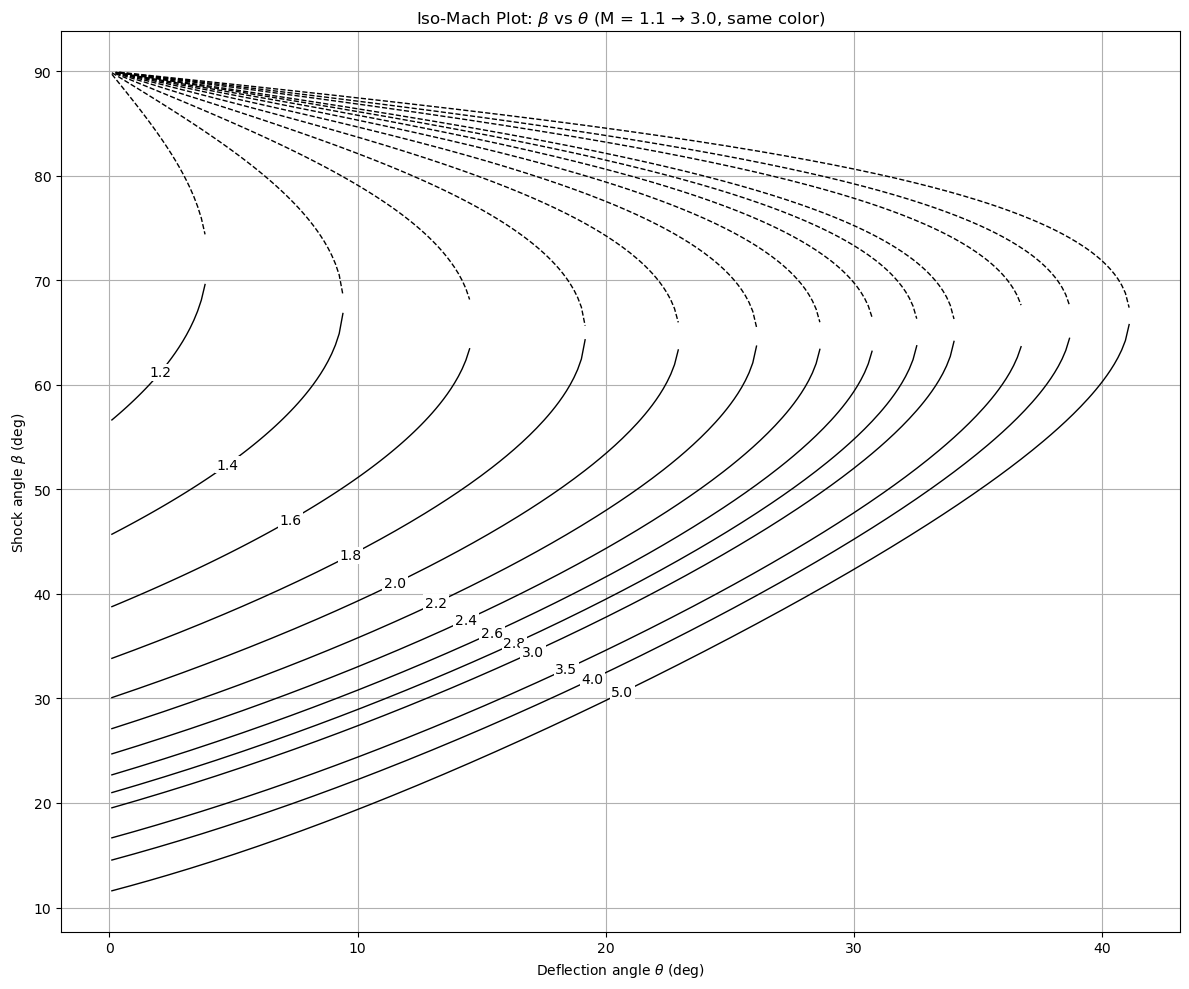
\includegraphics[width=\linewidth]{ressources/figures/compute_polaire.png}
        \caption{Computed polar}
    \end{minipage}
    \hfill
    \begin{minipage}[b]{0.45\linewidth}
        \centering
        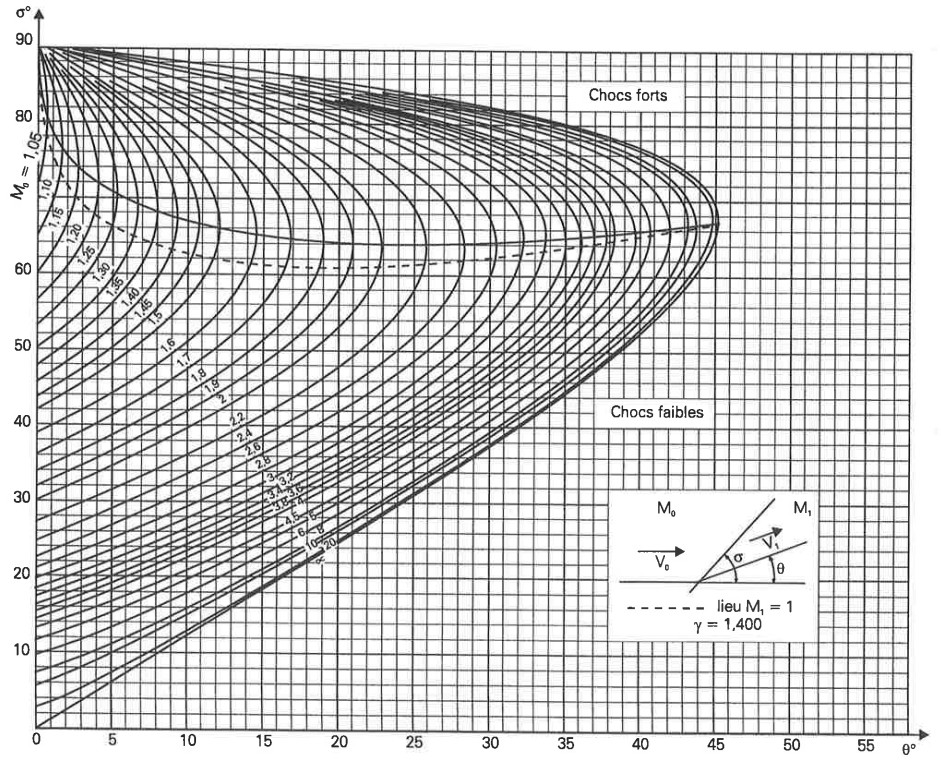
\includegraphics[width=\linewidth]{ressources/figures/supaero_polar.jpg}
        \caption{Published (Supaero) polar}
    \end{minipage}
    \label{fig:polar_comparison}
\end{figure}

The numerical and published polars agree closely. The slight discrepancy arises because the Supaero code uses a different plotting convention.

% ----- Linearized shock angle -----
\subsubsection{Linearized shock angle}

Because the exact solution is complex to compute, we also consider the small‐disturbance approximation. In the limit \(\theta \to 0\) with attached flow, the critical detachment condition is
\begin{align}
    M_\infty^2 \sin^2\beta_d - 1 &\approx 0
    \\
    \Longrightarrow\quad \beta_d &\approx \sin^{-1}\!\Bigl(\frac{1}{M_\infty}\Bigr).
\end{align}
\label{eq:beta_d}

This first‐order estimate corresponds to the weak solution. Note that the Mach angle \(\mu = \sin^{-1}(1/M_\infty)\) applies strictly to infinitesimal disturbances rather than finite shocks. We can now compare this linearized prediction with the exact numerical solution.

\begin{figure}[H]
    \centering
    \begin{minipage}[b]{0.45\linewidth}
        \centering
        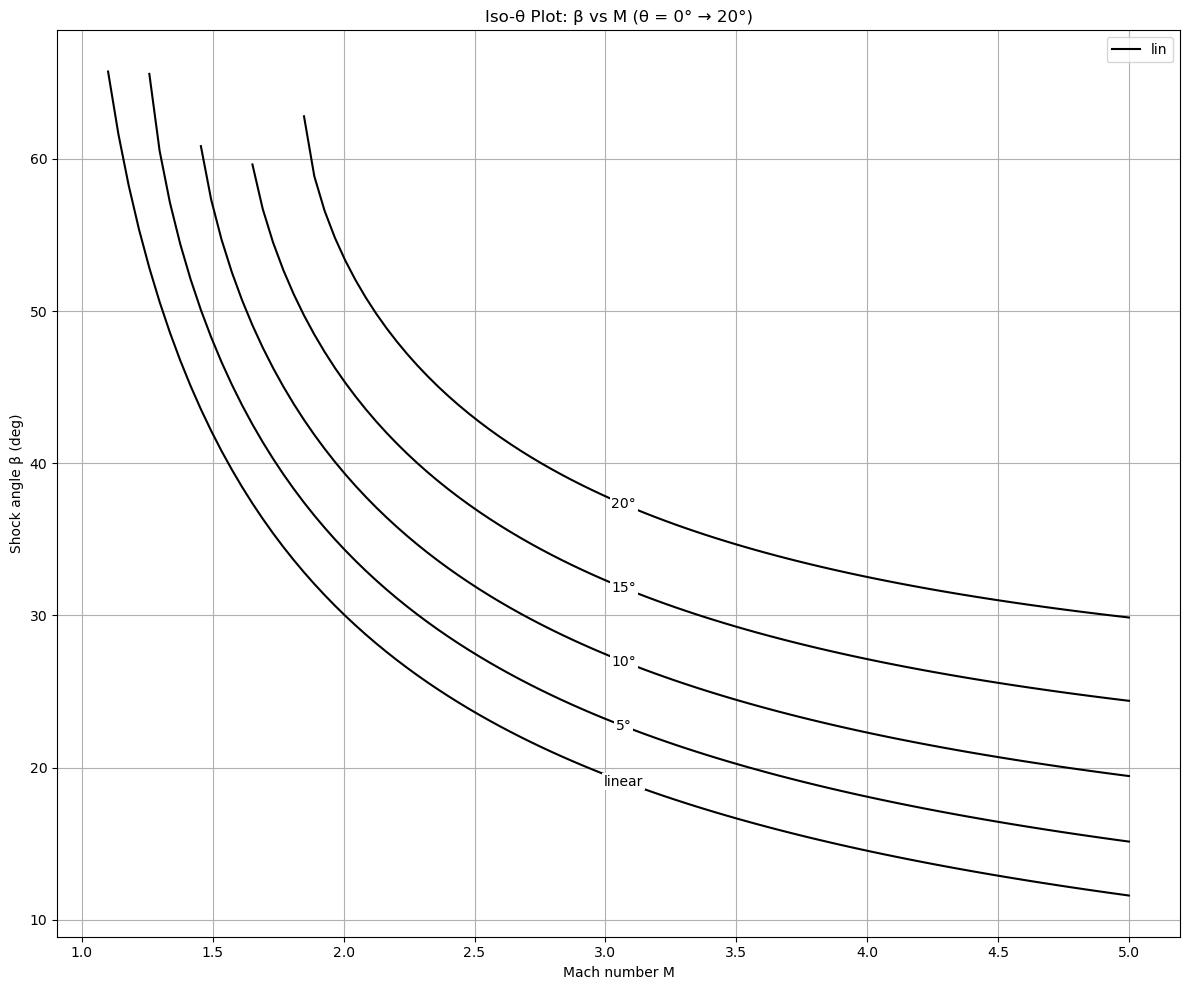
\includegraphics[width=\linewidth]{ressources/figures/linear_comparaison.png}
        \caption{Comparison of linearized and exact solutions}
    \end{minipage}
    \hfill
    \begin{minipage}[b]{0.45\linewidth}
        \centering
        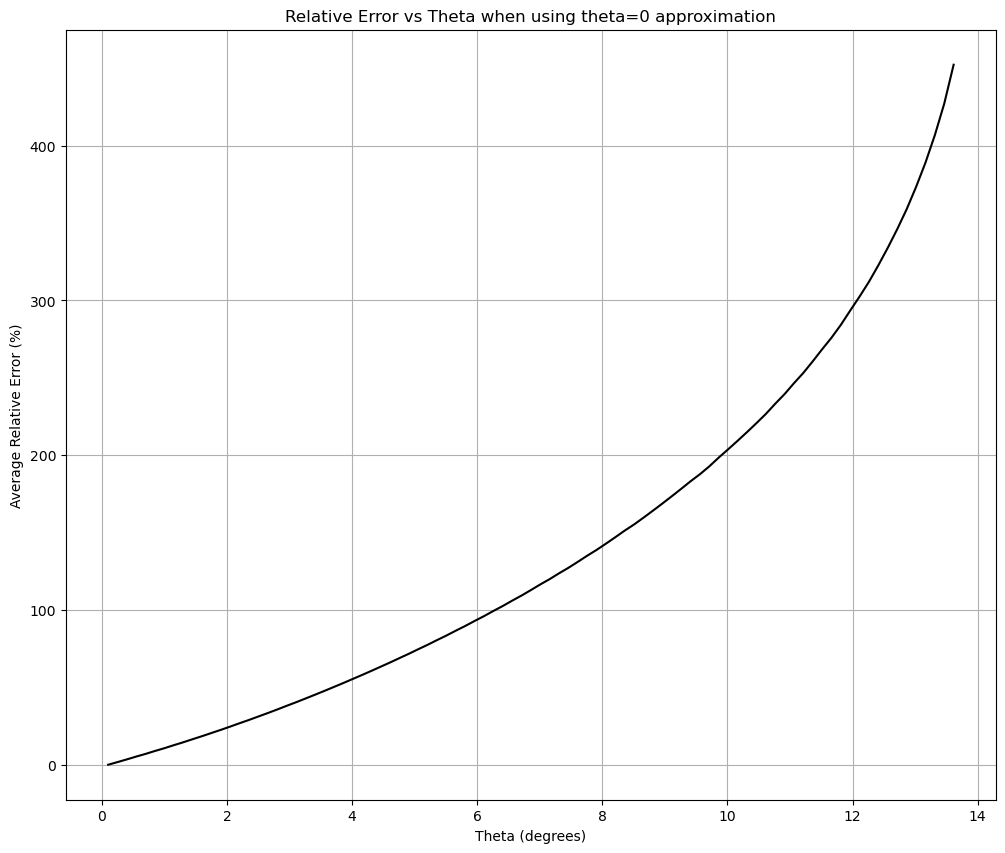
\includegraphics[width=\linewidth]{ressources/figures/linear_error.png}
        \caption{Error evolution}
    \end{minipage}
    \label{fig:linear_comparaison}
\end{figure}

As expected, the linearized solution matches the exact solution perfectly at \(\theta = 0\). The error increases exponentially with deflection angle but decreases as Mach number increases, converging to a constant value. This behavior explains the larger average error seen in Figure~\ref{fig:linear_comparaison}(b), while still capturing the overall trend of increasing error with deflection angle.
